\documentclass[ignorenonframetext, professionalfonts, hyperref={pdftex, unicode}]{beamer}

\usetheme{Copenhagen}
\usecolortheme{wolverine}

%Packages to be included
%\usepackage{graphicx}

\usepackage[russian]{babel}
\usepackage[utf8]{inputenc}
\usepackage[T1]{fontenc}

%%\usepackage[orientation=landscape, size=custom, width=16, height=9.75, scale=0.5]{beamerposter}

\usepackage{textcomp}

\usepackage{beamerthemesplit}

\usepackage{ulem}

\usepackage{verbatim}

\usepackage{ucs}


\usepackage{listings}
\lstloadlanguages{bash}

\lstset{escapechar=`,
	extendedchars=false,
	language=sh,
	frame=single,
	tabsize=2, 
	columns=fullflexible, 
%	basicstyle=\scriptsize,
	keywordstyle=\color{blue}, 
	commentstyle=\itshape\color{brown},
%	identifierstyle=\ttfamily, 
	stringstyle=\mdseries\color{green}, 
	showstringspaces=false, 
	numbers=left, 
	numberstyle=\tiny, 
	breaklines=true, 
	inputencoding=utf8,
	keepspaces=true,
	morekeywords={u\_short, u\_char, u\_long, in\_addr}
	}

\definecolor{darkgreen}{cmyk}{0.7, 0, 1, 0.5}

\lstdefinelanguage{diff}
{
    morekeywords={+, -},
    sensitive=false,
    morecomment=[l]{//},
    morecomment=[s]{/*}{*/},
    morecomment=[l][\color{darkgreen}]{+},
    morecomment=[l][\color{red}]{-},
    morestring=[b]",
}

\author[Epam]{{\bf Epam}\\Low Level Programming Department}

%\institution[EPAM]{EPAM}
%\logo{\includegraphics[width=1cm]{logo.png}}

\title{Введение в GNU/Linux\\Командная строка}

\begin{document}
\begin{frame}
 \frametitle{}
 \titlepage
\end{frame}

\section{Интерфейс командной строки}
\mode<all>{% Тема. Командная строка. 
% Показать примеры использования. Рассказать о преимуществах и недостатках в
% сравненни с графическим "оконным" интерфейсом. 
% Ознакомить с назначениме  эмулятора терминала и об реализациях.

\begin{frame}{Примеры использования командной строки}
	\begin{columns}
	\column{0.5\textwidth}
        \begin{itemize}
            \item чаты
            \item компьютерные игры Quake, DotA
            \item операционные системы
        \end{itemize}
	\column{0.5\textwidth}
	% insert picture of Quake 
    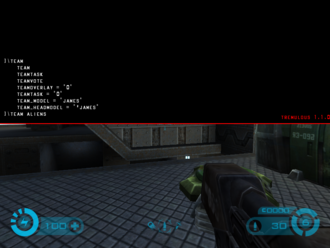
\includegraphics[height=0.4\textheight]{../../slides/cmdline/330px-Tremulous_console.png}
	\end{columns}
\end{frame}

\begin{frame}{Преимущества командной строки}
	\begin{itemize}
		\item Работа через сеть либо RS232
		\item Быстрый доступ к командам системы
		\item Легче отладка сообществом
		\item Легкость автоматизации
	\end{itemize}
\end{frame}

\begin{frame}{Недостатки командной строки}
	\begin{itemize}
		\item Oтсутствуют возможности обнаружения (discoverabililty)
		\item Необходимость изучения синтаксиса команд и запоминания сокращений.  (синтаксис может различаться)
		\item Без автодополнения, ввод длинных и содержащих спецсимволы параметров с клавиатуры может быть затруднительным
		\item Отсутствие «аналогового» ввода.
	\end{itemize}
\end{frame}

\begin{frame}{Эмуляторы терминала в графическом режиме}
	\begin{itemize}
		\item xterm
		\item rxvt
        \item gnome-terminal
        \item konsole
        \item Yakuake (Yet Another Kuake)
	\end{itemize}
\end{frame}
\note { 
Примеры приложений которые лучше выглядят в графическом режиме браузер,
редакторы видео и графики. Поэтому пользователь при работе, как правило,
совмещает оба интерфейса: использует графическое окружениe в сочетании с
интерфейсом командной строки. 
В графическом окружении интерфейса командной строки предоставляют приложения -
эмуляторы терминала. 
реализации - для графической системы X Window xterm, rxvt. Для GNOME
gnome-terminal, для KDE konsole, Yakuake (Yet Another Kuake выезжает по нажатии
тильды ~ как Quake)  
Дополнительные замечания:
Терминал - устройство для ввода вывода информации, уже устарел.
Графические приложения можно запускать из командной строки. 
}
}

\section{ Командная оболочка(shell) }
\begin{frame}
\frametitle{}
 \begin{center}
   {\Large Командная оболочка(shell) }
 \end{center}
\end{frame}

\mode<all>{\begin{frame}[fragile]{Определение(не совсем формальное)}
	\textbf{Shell} -- приложение, обеспечивающее выполнение других приложений и их взаимодействие, а также представляющая услуги командной строки. 
	\begin{center}
	 или
	\end{center}
	\textbf{Shell} -- приложение, обеспечивающее доступ к основным функциям ядра.

	\pause
	\vspace{0.5in}
	Пример shell из Windows-world -- cmd.exe
	\vspace{0.5in}

	Минимальный дистрибутив Linux -- ядро + shell 

\end{frame}

\begin{frame}[fragile]{Основные типы shell в Unix}
  \begin{itemize}
    \item Bourne shell совместимые
      \begin{itemize}
        \item \textbf{sh} исходная bourne shell (Steve Bourne, 1978)
        \item \textbf{ksh} Korn shell (David Korn, 1983)
        \item \textbf{ash} $[$BSD$]$ Almquist shell (Kenneth Almquist,1989)  
        \item \textbf{bash} $[$GPL$]$ Bourne-again shell (Brian Fox, 1989)
        \item \textbf{zsh} $[$BSD$]$ Z shell (Paul Falstad,1990)
        \item \textbf{/bin/sh} Указывает на POSIX-совместимую shell
      \end{itemize}
  \item C shell совместимые
      \begin{itemize}
        \item \textbf{csh}  Исходная С shell (Bill Joy, 1978)
        \item \textbf{tcsh} $[$BSD$]$ TENEX C shell (Ken Greer, 1981)
       \end{itemize}
  \end{itemize}
\end{frame}

\begin{frame}[fragile]{Маленькое упражнение}
\begin{lstlisting}[language=bash]
cat /etc/shells
ls -l <filename> # для каждого элемента /etc/shells
readlink -e <filename> 
\end{lstlisting}
\end{frame}


}

\section{ Документация }
\begin{frame}
\frametitle{}
 \begin{center}
   {\Large Help }
 \end{center}
\end{frame}
\mode<all>{
\begin{frame}[fragile]{Как правильно задавать вопросы}
From FAQ How To Ask Questions The Smart Way
Before You Ask
  \begin{itemize}
	  \item Try to find an answer by reading the manual.
	  \item Try to find an answer by reading a FAQ.
	  \item Try to find an answer by searching the archives of the forum you plan to post to.
	  \item Try to find an answer by searching the Web.
	  \item Try to find an answer by inspection or experimentation.
	  \item Try to find an answer by asking a skilled friend.
	  \item If you're a programmer, try to find an answer by reading the source code.
    \end{itemize}
\end{frame}


\begin{frame}[fragile]{Источники получение помощи}
  \begin{itemize}
    \pause
    \item \textbf{man} - помощь по внешним командам
    \pause
    \item \textbf{help} - встроенная помощь по внутренним командам bash (также man bash)
    \pause
    \item \textbf{info} - расширенная помощь по некоторым командам (texinfo format)
     \begin{block}{Упражнение. Работа с командой info}
        \begin{itemize}
        \item   Попробовать {\tt info coreutils}
        \item   Справка по навигации -- нажать h
        \end{itemize}
	 \end{block}
		\begin{block}{Упражнение. Другие источники помощи.}
			\begin{lstlisting}
            help 
            help help
            man -h
            info --help
			\end{lstlisting}
		\end{block}
  \end{itemize}
\end{frame}

\begin{frame}[fragile]{Основное о man}
\begin{columns}
	\column{2.5in}
		\begin{itemize}
			\item Прочитайте {\tt man man} !
			\item apropos, аналог {\tt man -k <слово>}
            \item whatis, аналог {\tt man -f <слово>} 
			\item Разделы (sections)
				\begin{itemize}
					\item[1] Основная секция(юзерские программы)
					\item[2] Syscalls
					\item[3] С library
					\item[5] Конфигурационные файлы
					\item[8] Системные службы
				\end{itemize}
		\end{itemize}
	  \textbf{Замечание}

	  Обычно внутри страницы работает поиск с помощью '/'
	\pause 
	
	\column{1in}
		\begin{block}{Попробовать}
			\begin{lstlisting}
man -k intro or apropos
man -f intro or whatis
man 3 intro
man 1 intro
man -wa intro
			\end{lstlisting}
		\end{block}
	\end{columns}
\end{frame}


%\begin{frame}[fragile]{Чему научились}
%  \begin{itemize}
%  \item Как спрашивать у сообщества
%  \item Умеем использовать 3 источника получения информации man, info, help
%  \item Как перемещаться по страницам помощи info и man
%  \item Иcкать в системе помощи man и запрашивать из одного из 8-ми разделов 
%  \end{itemize}
%\end{frame}
}

\section{ Навигация по файловой системе}
\begin{frame}
\frametitle{}
 \begin{center}
   {\Large Навигация по файловой системе }
 \end{center}
\end{frame}
\mode<all>{\begin{frame}{Файловая структура}
	
	{\center "Дерево внутри дома?" (c) Шрек}
		
	\begin{columns}
	\column{0.2\textwidth}
		\includegraphics[height=0.8\textheight]{../../slides/fs/01-lhs.png}
		
	\column{0.7\textwidth}
		\begin{itemize}
			\item Директории
			\item Обычные файлы
			\item Симлинки
			\item Хардлинки
			\item Файлы устройств
			\item FIFO
			\item сокеты
		\end{itemize}
	\end{columns}
\end{frame}
}

\mode<all>{\begin{frame}{Навигация по файловой системе}
      \begin{itemize}
		  \item {\tt ls} -- список файлов в (текущей по умолчанию) директории (man ls)
		  \item {\tt cd} -- смена текущей директории (help cd)
		  \item {\tt pwd} -- имя текущей директории (help pwd)
      \end{itemize}
\end{frame}

\begin{frame}[fragile]{Команды для работы с файлами}
	\begin{itemize}
		\begin{columns}
		\column{0.2\textwidth}
			\item touch
			\item ln
			\item mkdir
			\item mknod
			\item mkfifo
		\column{0.2\textwidth}
			\item cp
			\item mv
			\item install
			\item rm
			\item rmdir
			\item file
		\column{0.4\textwidth}
			\begin{block}{Упражнение}
				\begin{enumerate}
					\item Создать иерархию директорий
						\begin{lstlisting}
dir1/dir1.1/dir1.1.1
dir1/dir1.2/dir1.2.1
dir1/dir1.2/dir1.2.2
						\end{lstlisting}
					\item Внутри каждой создать файл
					\item Удалить все созданное
				\end{enumerate}
			\end{block}
		\end{columns}
	\end{itemize}
\end{frame}


}


\section{ Дополнительные возможности оболочки}
\mode<all>{\begin{frame}{Важные аббревиатуры внутри командной строки}
  \begin{itemize}
    \item Для директорий
      \begin{itemize}
        \item {\tt $\sim$} Домашняя директория
        \item {\tt $\sim$<username>} Домашняя директория пользователя
        \item {\tt ..} Родительская директория
        \item {\tt .} Текущая директория
      \end{itemize}
      \pause  
    \item Wildcards
      \begin{itemize}
        \item {\tt *} Любой набор символов {\tt file*txt : file1.txt filefilefiletxt}
        \item {\tt $[$<список>$]$ } символ из заданного набора
        \item {\tt ?} любой один символ
      \end{itemize}

  \end{itemize}
\end{frame}       

\begin{frame}{Горячие клавиши}
  \begin{itemize}
    \item \textbf{Tab} -- дополнение текущей команды
      \pause
    \item История команд
      \begin{itemize}
        \item Клавиши курсора -- навигация по истории
        \item Ctrl-R -- поиск в истории по фрагменту
        \item Ctrl-O (после выполнения вставить следующую команду из истории)
        \item Команда {\tt history}
      \end{itemize}
    \item Навигация

  \end{itemize}
\end{frame}

\begin{frame}{Переменные окружения}
  \begin{itemize}
    \item {\tt HOME}
    \item {\tt PWD}
    \item {\tt LANG}
    \item {\tt LD\_LIBRARY\_PATH}
    \item {\tt SHELL}
    \item {\tt TERM}
    \item {\tt DISPLAY}
  \end{itemize}

  Контроль

  \begin{itemize}
    \item export {\tt export VAR=value}
    \item declare -x
    \item echo 
  \end{itemize}

  Переменные окружения наследуются при создании нового процесса
\end{frame}

%\begin{frame}{Настройки bash и кастомизация}
%  \begin{itemize}
%    \item Login shell
%      \begin{itemize}
%        \item {\tt /etc/profile}
%        \item {\tt $\sim$/.profile }
%      \end{itemize}
%    \item Обычная интерактивная shell
%      \begin{itemize}
%        \item {\tt /etc/bash.bashrc}
%        \item {\tt $\sim$/.bashrc}
%      \end{itemize}
%  \end{itemize}
%
%  Полезные команды
%  \begin{itemize}
%    \item {\tt alias}
%    \item {\tt export PATH=}
%    \item {\tt Определение функции}
%    \item {\tt shopts}
%  \end{itemize}
%
%\end{frame}


}


\begin{frame}{Задание на дом}
\begin{block}{}
vimtutor ru
\end{block}
\end{frame}

\end{document}

